\section{Deep Learning}

Deep Learning is a powerful subset of Machine Learning that focuses on automatically learning the most relevant features from raw data. 
Unlike traditional Machine Learning methods, which rely on manually extracted features, Deep Learning models take raw input and learn hierarchical representations directly. 
This capability makes Deep Learning highly effective for complex tasks but also introduces challenges in terms of model complexity and interpretability. 
While Deep Learning often outperforms traditional Machine Learning, it is not always the best choice (especially when domain expertise allows for efficient manual feature extraction). 
Additionally, Deep Learning models are computationally more demanding and require significantly more resources to train and deploy.

A typical Convolutional NN (CNN) consists of two main types of layers: convolutional layers and fully connected layers.

\subsection{Convolutional layer}
Each convolutional layer typically includes several key components:
\begin{itemize}
    \item \textit{Convolutional filters} (trainable): these apply spatial operations to the input, with parameters such as filter size, number of filters, and stride.
    \item \textit{Activation functions}: nonlinear transformations introduce nonlinearity into the model, enabling it to learn complex relationships.
    \item \textit{Normalization} (trainable) : optional techniques like batch normalization improve training stability and performance.
    \item \textit{Pooling}: reduces spatial dimensions, helping to control overfitting and computational costs.
\end{itemize}
Consider an RGB image with dimensions $H\times W \times C$, where $H$ and $W$ represent the height and width of the image, and $C$ denotes the number of channels (3 for RGB, 1 for gray scale).
Convolutional filters have dimensions $R\times S\times C$, where $R$ and $S$ are the filter's spatial dimensions, and $C$ matches the number of channels in the input image.

\begin{figure}[H]
    \centering
    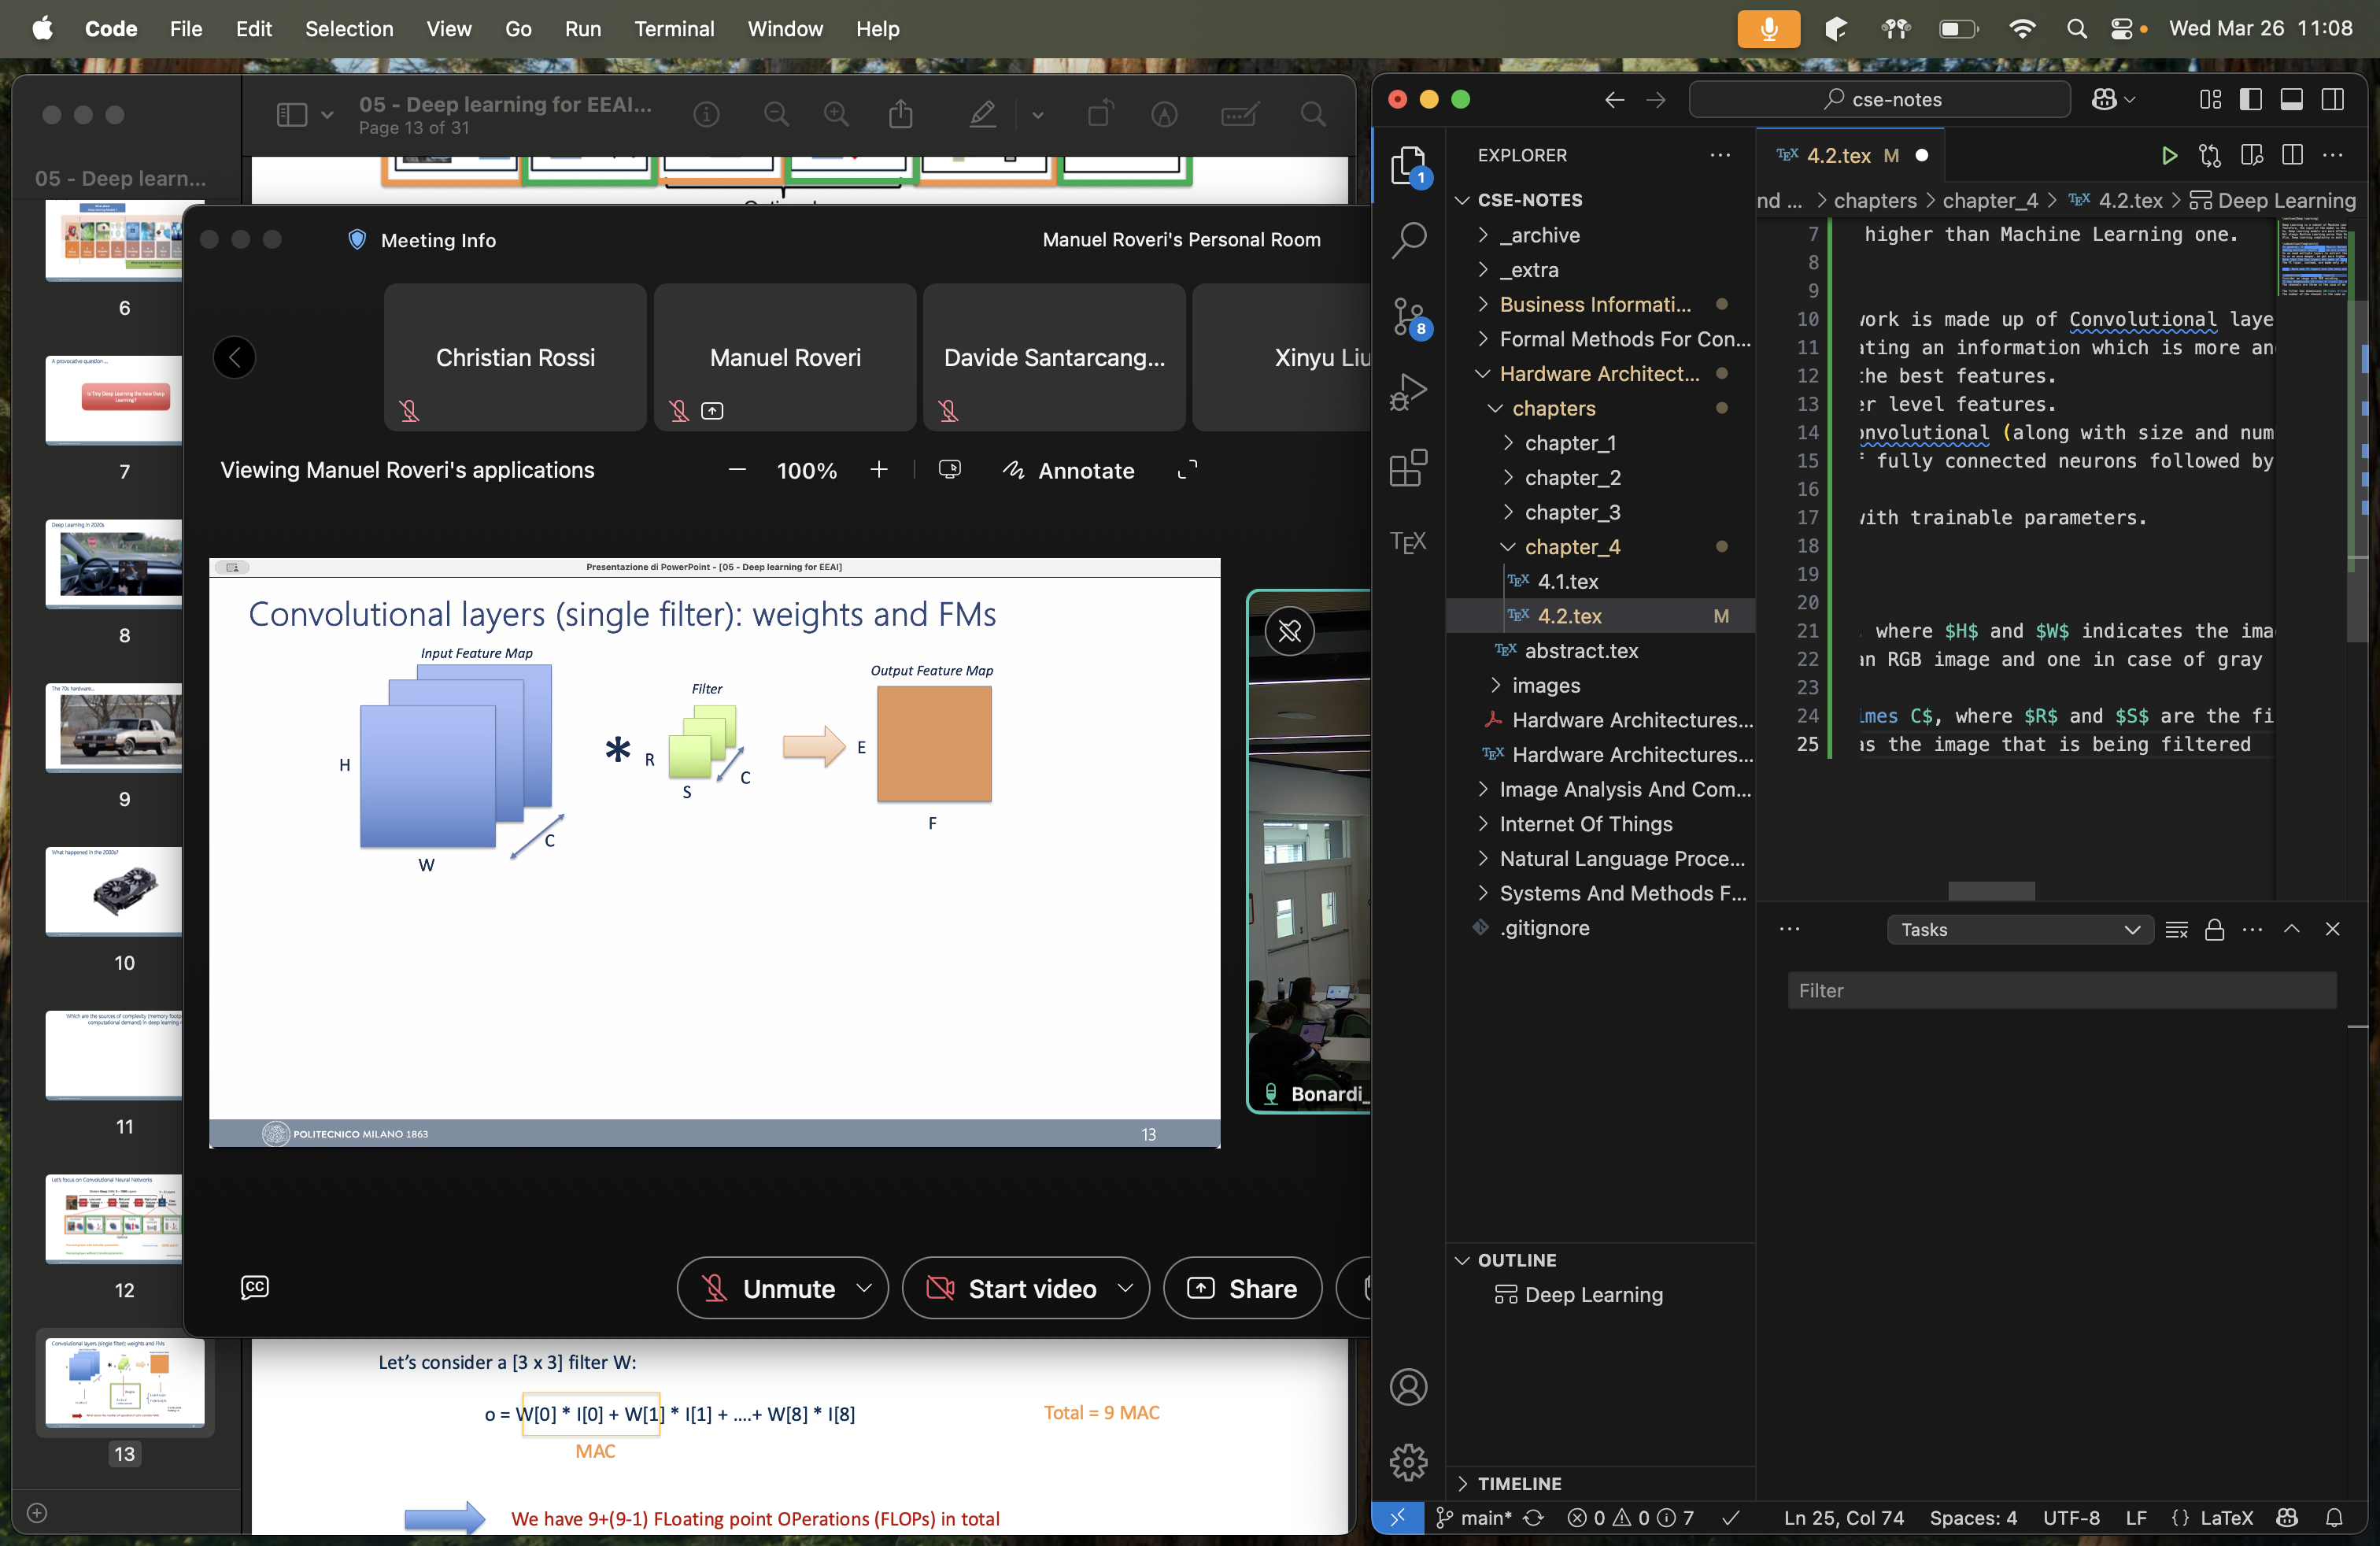
\includegraphics[width=0.5\linewidth]{images/eeai7.png}
    \caption{Convolutional layer}
\end{figure}

The output of applying a filter to the image has dimensions $E\times F$, with the number of channels equal to the number of filters used. 
The exact size of the output depends on the filter dimensions, the stride ($U$), and whether padding is applied. 
Specifically, with no padding we have :
\[\begin{cases}
    E=\frac{H-R+U}{U} \\
    F=\frac{W-S+U}{U}
\end{cases}\]
\noindent Each filter has $R\times S \times C+1$ parameters (including the bias term). 
Even with a single filter, the number of parameters can grow rapidly, especially for large images.

\paragraph*{Computational demand}
The computational cost of a convolutional layer is primarily determined by the number of multiply-and-accumulate (MAC) operations.
For a single $3\times 3$ filter, there are 9 MACs (one for each weight) and a total of $9+(9-1)=17$ floating-point operations (FLOPs). 
In general:
\[1\text{ MAC}\approx 2\text{ FLOPS}\]
For a convolutional layer with $M$ filters, the total number of MAC operations is:
\[\text{MAC}=E\times F\times R\times S\times C\times M\]
\noindent Here, where $E\times F$ is the output size, $R\times S$ is the filter size, $C$ is the number of input channels, and $M$ is the number of filters.

\subsection{Fully connected layer}
Fully connected layers consist of densely connected neurons followed by activation functions. 
These layers are responsible for combining the high-level features extracted by the convolutional layers to make predictions.

In a fully connected layer, each neuron receives input from all neurons in the previous layer. 
Given an input layer with $H$ neurons and a fully connected layer with $W$ neurons, the total number of parameters is $H\times W+W$, where the additional $W$ accounts for the bias terms.
\begin{figure}[H]
    \centering
    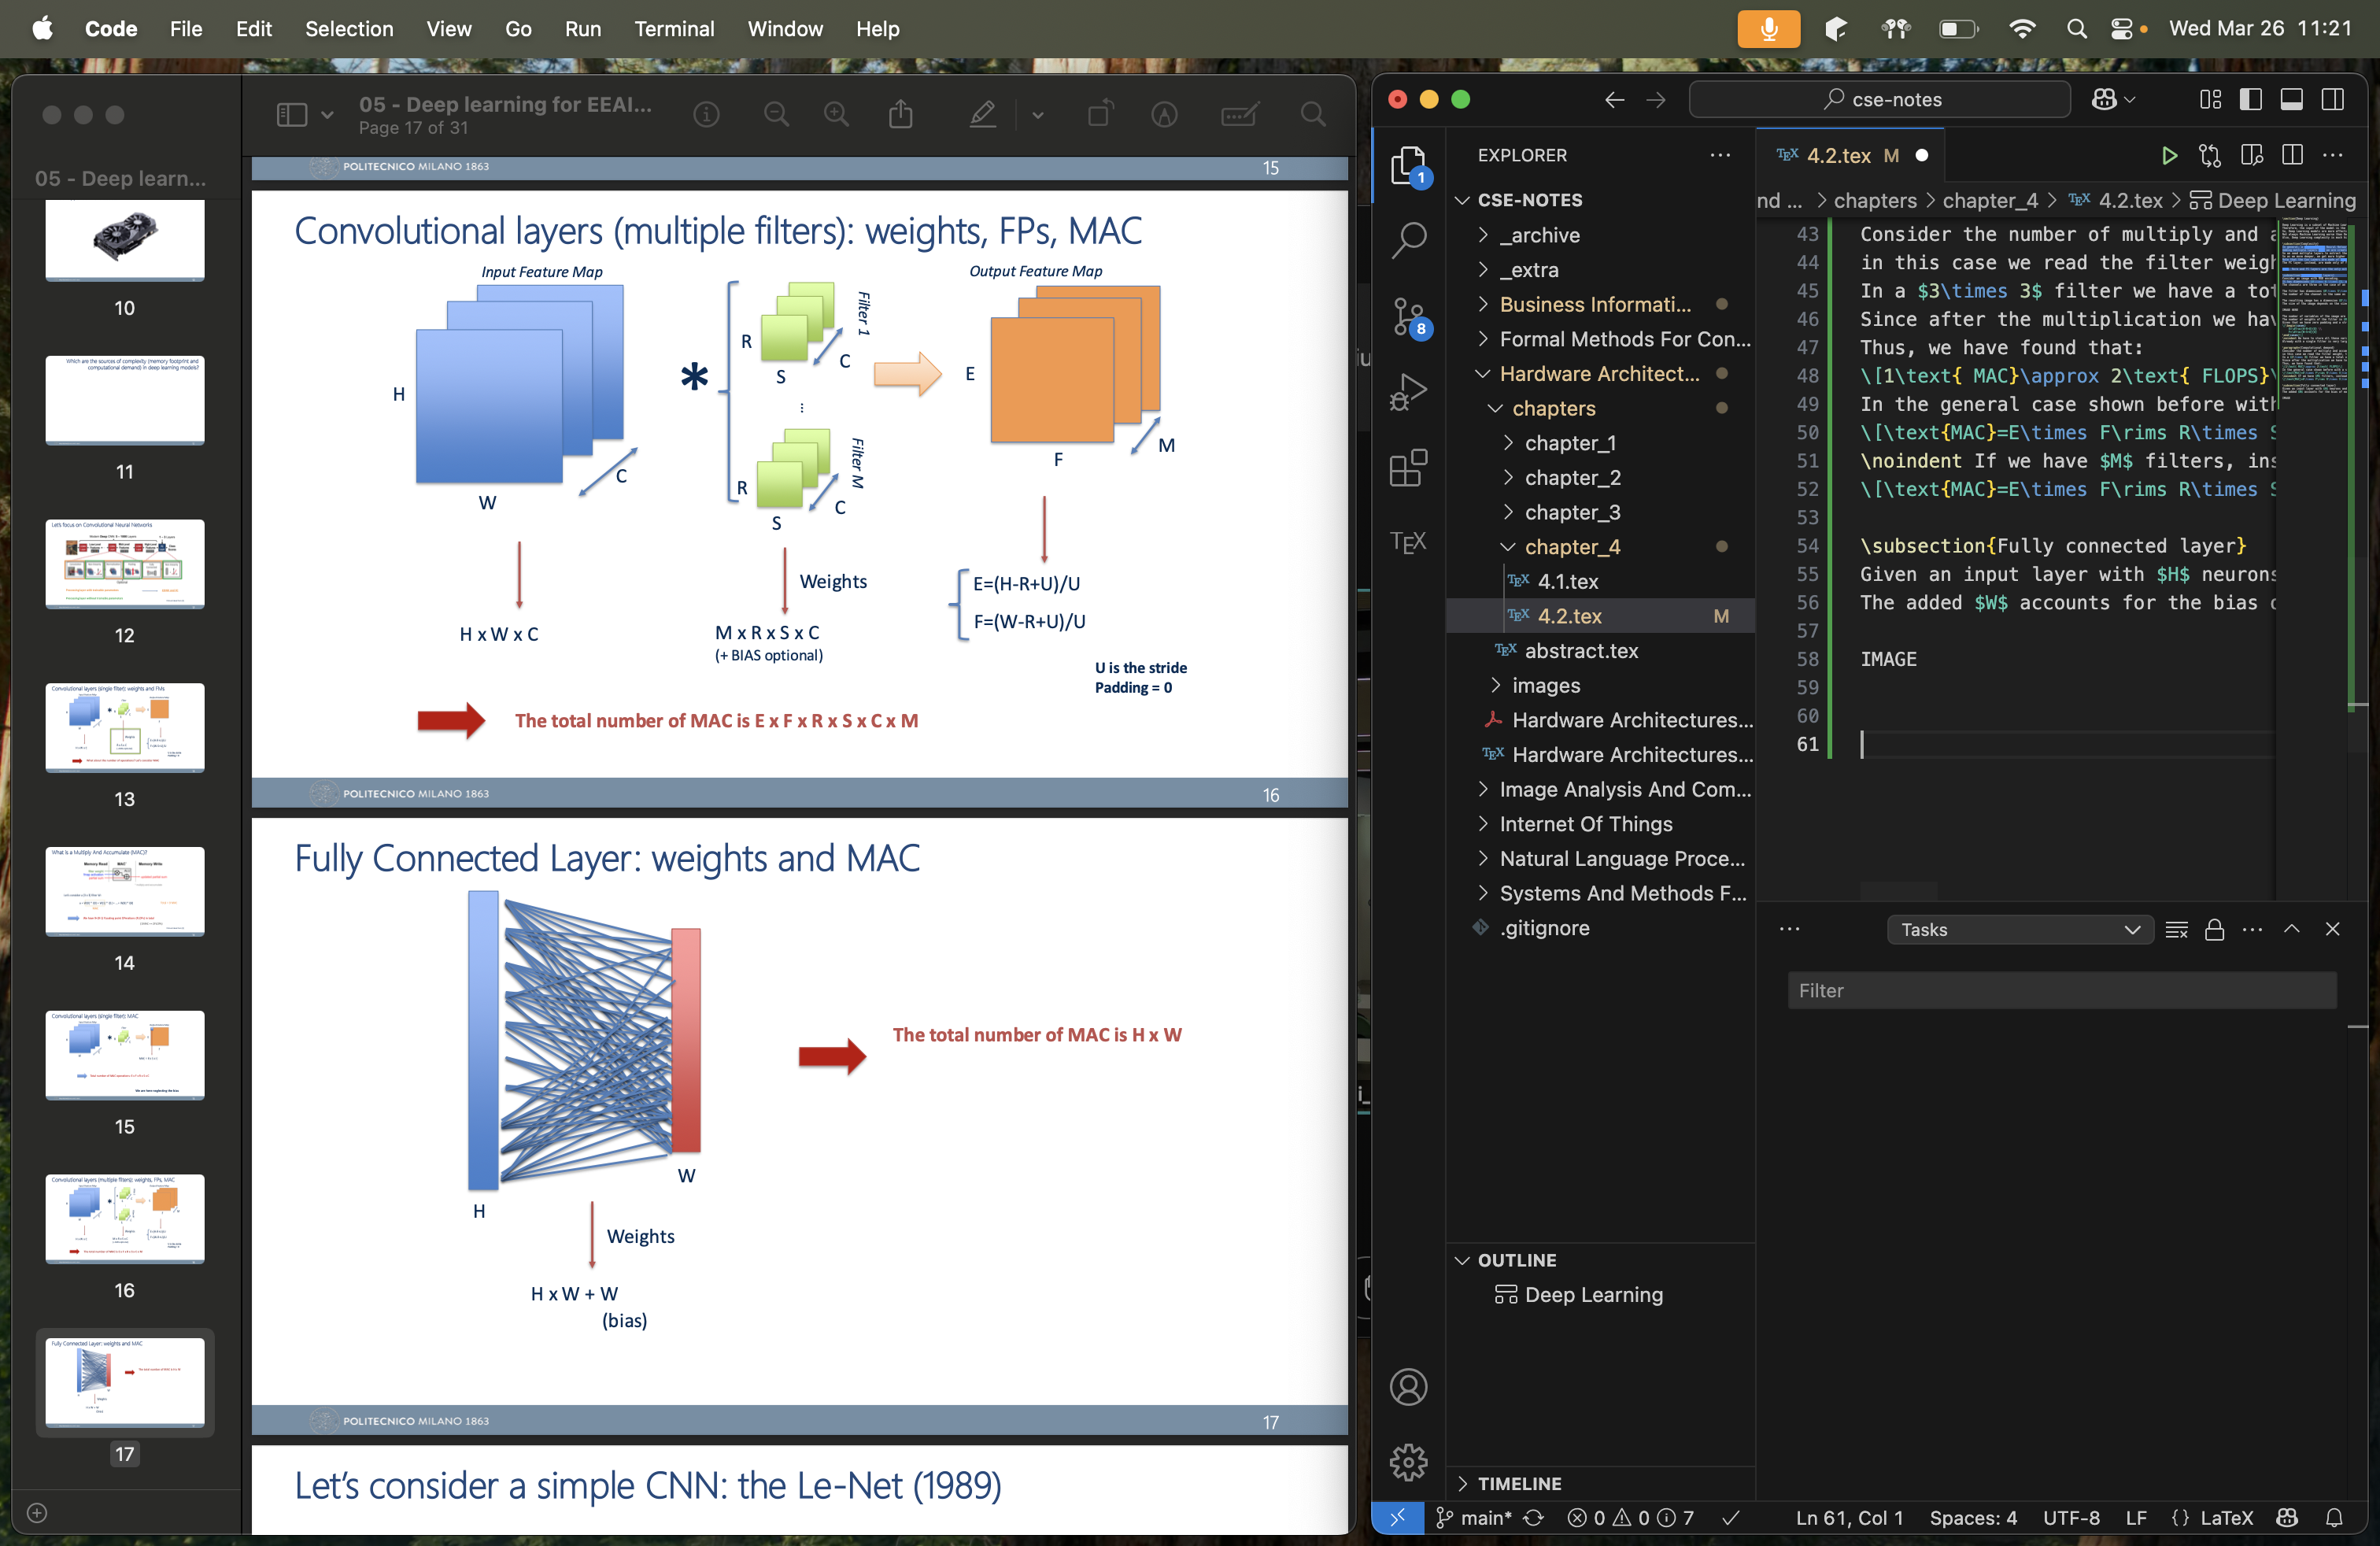
\includegraphics[width=0.25\linewidth]{images/eeai8.png}
    \caption{Fully connected layer}
\end{figure}
The computational cost is proportional to the number of MAC operations:
\[\text{MAC}=H\times W\]

\subsection{Memory occupation}
Convolutional layers generally occupy less memory than fully connected layers due to their sparse connectivity and parameter sharing. 
However, they tend to require more MAC operations, making them computationally expensive. 
Each parameter occupies approximately 4 bytes, so the total memory footprint of a NN is determined by the number of parameters multiplied by this value.
Additionally:
\begin{itemize}
    \item The firmware for the device typically requires around $10\text{ kB}$.
    \item Input, output, and intermediate feature maps must also be stored in memory. 
        Their size is given by:
        \[H\times W \times C\times 4\]
        This can be a significant bottleneck, especially for large inputs or deep networks.
\end{itemize}
\noindent Modern architectures often reduce the number of fully connected layers while increasing the depth and efficiency of convolutional layers.

\subsection{Tiny Deep Learning}
To address the challenges posed by the size and complexity of NNs, we can explore several strategies to make them more efficient and suitable for resource-constrained environments:

\begin{itemize} 
    \item \textit{Redesigning CNN architectures}: develop new, lightweight layers that reduce the overall computational burden while maintaining performance. 
        This involves creating compact network structures that achieve high efficiency without compromising too much on accuracy.
    \item \textit{Approximate computing}: embrace techniques that trade off a small amount of precision for significant gains in computational speed and memory usage. 
        By allowing minor inaccuracies in calculations, we can drastically improve the efficiency of both training and inference processes.  
    \item \textit{Code optimization for embedded systems}: fine-tune the implementation of Deep Learning models to better suit the hardware constraints of embedded devices. 
        This includes optimizing memory usage, leveraging hardware-specific instructions, and minimizing latency to ensure smooth operation on edge devices.
\end{itemize}